%% When submitting camera ready or to TAPS, please change the command
%% to \documentclass[sigconf]{acmart} or whichever template is required
%% for your publication.
%%
%%
% \documentclass[sigconf]{acmart}
\documentclass[manuscript,screen,review]{acmart}
%%
%% \BibTeX command to typeset BibTeX logo in the docs
\AtBeginDocument{%
  \providecommand\BibTeX{{%
    Bib\TeX}}}



% TODO: What should we write in the following?
%% Rights management information.  This information is sent to you
%% when you complete the rights form.  These commands have SAMPLE
%% values in them; it is your responsibility as an author to replace
%% the commands and values with those provided to you when you
%% complete the rights form.
%\setcopyright{acmlicensed}
%\copyrightyear{2026}
%\acmYear{2026}
%\acmDOI{XXXXXXX.XXXXXXX}
%% These commands are for a PROCEEDINGS abstract or paper.
%\acmConference[Conference acronym 'XX]{Make sure to enter the correct
%  conference title from your rights confirmation email}{June 03--05,
%  2018}{Woodstock, NY}
%%
%%  Uncomment \acmBooktitle if the title of the proceedings is different
%%  from ``Proceedings of ...''!
%%
%%\acmBooktitle{Woodstock '18: ACM Symposium on Neural Gaze Detection,
%%  June 03--05, 2018, Woodstock, NY}
%\acmISBN{978-1-4503-XXXX-X/2018/06}

% Rights management information
\setcopyright{none} % no copyright assigned yet
\copyrightyear{2026}
\acmYear{2026}
\acmDOI{} % DOI not assigned yet

% Conference information (to fill in after acceptance)
\acmConference[]{}{}{} % leave empty until acceptance
%\acmBooktitle{} % optional, fill after acceptance
\acmISBN{} % leave empty



%%
%% Submission ID.
%% Use this when submitting an article to a sponsored event. You'll
%% receive a unique submission ID from the organizers
%% of the event, and this ID should be used as the parameter to this command.
%%\acmSubmissionID{123-A56-BU3}

%%
%% For managing citations, it is recommended to use bibliography
%% files in BibTeX format.
%%
%% You can then either use BibTeX with the ACM-Reference-Format style,
%% or BibLaTeX with the acmnumeric or acmauthoryear sytles, that input
%% support for advanced citation of software artefact from the
%% biblatex-software package, also separately available on CTAN.
%%
%% Look at the sample-*-biblatex.tex files for templates showcasing
%% the biblatex styles.
%%

%%
%% The majority of ACM publications use numbered citations and
%% references.  The command \citestyle{authoryear} switches to the
%% "author year" style.
%%
%% If you are preparing content for an event
%% sponsored by ACM SIGGRAPH, you must use the "author year" style of
%% citations and references.
%% Uncommenting
%% the next command will enable that style.
%%\citestyle{acmauthoryear}


%%
%% end of the preamble, start of the body of the document source.

\usepackage{booktabs}
\usepackage{caption}
\usepackage{threeparttable}
\captionsetup[table]{skip=5pt} % Ajusta el 'skip' a los puntos que desees
\begin{document}

%%
%% The "title" command has an optional parameter,
%% allowing the author to define a "short title" to be used in page headers.
\title{Monitoring and Understanding Notebook-Based Learning with Jupyter}
\subtitle{A Dashboard for Student Self-Assessment}

%%
%% The "author" command and its associated commands are used to define
%% the authors and their affiliations.
%% Of note is the shared affiliation of the first two authors, and the
%% "authornote" and "authornotemark" commands
%% used to denote shared contribution to the research.

\author{Arturo Olivares Martos}
\email{arturoolivares@correo.ugr.es}
\email{arturo.olivares@stud.uni-due.de}
\affiliation{%
  \institution{Universidad de Granada}
  \city{Granada}
  \country{Spain}
}

\author{Lisa Pawlowski}
\email{lisa.pawlowski.99@stud.uni-due.de}
\affiliation{%
  \institution{University of Duisburg-Essen}
  \city{Duisburg}
  \country{Germany}
}

%%
%% By default, the full list of authors will be used in the page
%% headers. Often, this list is too long, and will overlap
%% other information printed in the page headers. This command allows
%% the author to define a more concise list
%% of authors' names for this purpose.
% \renewcommand{\shortauthors}{Olivares Martos and Pawlowski}

%%
%% The abstract is a short summary of the work to be presented in the
%% article.
\begin{abstract}
  As programming becomes increasingly integrated into scientific and educational workflows, the need to understand how users interact with computational notebooks has grown. This project introduces a JupyterLab dashboard extension that monitors and visualizes notebook activity, including notebook openings, cell execution outcomes, errors, and retries. The system produces summary statistics and visual timelines that portray how the workflow unfolds. The dashboard is intended to be used by students for self-assessment and awareness of their coding patterns. A survey was conducted to gather user feedback on the dashboard's usability and usefulness. The insights gained from this evaluation serve as a pilot study, establishing a baseline for the tool's usability and paving the way for future research on its pedagogical impact.
\end{abstract}

%%
%% The code below is generated by the tool at http://dl.acm.org/ccs.cfm.
%% Please copy and paste the code instead of the example below.
%%
\begin{CCSXML}
<ccs2012>
   <concept>
       <concept_id>10010405.10010489.10010491</concept_id>
       <concept_desc>Applied computing~Interactive learning environments</concept_desc>
       <concept_significance>500</concept_significance>
       </concept>
   <concept>
       <concept_id>10003120.10003145.10011769</concept_id>
       <concept_desc>Human-centered computing~Empirical studies in visualization</concept_desc>
       <concept_significance>500</concept_significance>
       </concept>
 </ccs2012>
\end{CCSXML}

\ccsdesc[500]{Applied computing~Interactive learning environments}
\ccsdesc[500]{Human-centered computing~Empirical studies in visualization}

%%
%% Keywords. The author(s) should pick words that accurately describe
%% the work being presented. Separate the keywords with commas.
\keywords{
  Jupyter Notebooks,
  Learning Analytics,
  Educational Dashboards,
  Student Self-Assessment,
  Instructor Insights,
  Interactive Coding Environments
}

\received{26 February 2026}
%\received[revised]{}
%\received[accepted]{}


%%
%% This command processes the author and affiliation and title
%% information and builds the first part of the formatted document.
\maketitle

\section{Introduction}
Computational notebooks such as Jupyter have become central tools in scientific computing, teaching, and data analysis. Their interactive structure—mixing narrative text, code, and visual output—makes them highly suitable for inquiry-based learning in programming education~\cite{perkel2018jupyter}. Yet despite their pedagogical advantages, instructors often lack visibility into how students actually work within these environments. Students, on the other hand, often have little opportunity to reflect on their own workflow, error patterns, or problem-solving behavior. Research in programming education consistently shows that learners repeat similar types of mistakes, struggle to identify the sources of their errors, and often adopt inefficient trial-and-error strategies. At the same time, teachers typically only see final code submissions, which provide limited insight into the learners' process~\cite{robinson2022error}. This creates a gap between the correctness of the final code and the path the student took to reach it. Understanding this process is crucial to improve teaching interventions and help students develop their metacognitive skills.

Learning dashboards have been shown to enhance students' self-awareness, foster reflection, and offer instructors actionable insights into learner behavior. However, the majority of existing dashboards focus on high-level learning management system data rather than fine-grained programming behavior within computational notebooks~\cite{paulsen2024learning}. To bridge this gap, it is first necessary to develop tools that translate raw notebook interactions into meaningful visualizations and, crucially, to evaluate whether students perceive such tools as useful and easy to integrate into their workflow.

This project addresses this gap by designing a JupyterLab dashboard extension capable of tracking detailed notebook interactions, such as cell-level execution histories and error patterns. The primary objective of this study is to evaluate the usability, perceived usefulness, and cognitive workload of this newly developed dashboard from a learner's perspective. By focusing on the user experience (UX) and technology acceptance, this research aims to determine if the proposed system provides a viable foundation for supporting self-reflection in programming education.
To evaluate the system, an exploratory study was conducted with 22 students. Participants engaged with the dashboard while solving Python exercises and subsequently provided feedback through standardized instruments, including the System Usability Scale (SUS), the Technology Acceptance Model (TAM), and the NASA Task Load Index (NASA-TLX)~\cite{germanupa_sus, davis1989technology, hart1988development}. This approach allows for a comprehensive assessment of whether the dashboard meets the needs of students and identifies potential barriers to its adoption. The findings contribute to the field of learning analytics by providing empirical evidence on the design and acceptance of fine-grained, student-centered reflection tools in computational environments.


\section{Related Work}

Computational notebooks have gained significant relevance in education and research, and recent work has explored how learners interact within these environments. A growing body of research shows that while notebooks support exploratory coding and flexible workflows, they also introduce challenges for understanding the learning process at a fine-grained level. Systems designed to capture cell-level interaction data, such as execution patterns, time on task and navigation behavior demonstrate that detailed traces can reveal iterative retries, hesitation, and fragmented workflows that remain invisible in final notebook submissions~\cite{cai2025jupyter}. However, existing approaches of this type are primarily designed for instructor-facing analytics and do not address how such data could support student reflection or metacognitive skill development.

In programming education more broadly, research consistently shows that novice programmers struggle with error identification and debugging, often relying on unsystematic trial-and-error strategies and showing difficulty in locating the source of errors~\cite{robinson2022error}. Additional studies highlight that notebook environments exhibit recurring categories of bugs, suggesting that the structure of notebooks can reinforce certain misunderstandings or error patterns~\cite{de2022bug}. These findings underline the importance of tools capable of making the coding process more transparent and helping learners understand not only the errors they make, but also how they arrive at those errors. However, for such tools to be effective, they must be seamlessly integrated into the student's workflow without increasing cognitive burden~\cite{corrin2014exploring}.

Learning analytics dashboards have been widely explored as mechanisms for supporting student awareness, self-regulation, and instructional decision-making. Systematic reviews show that dashboards can enhance metacognitive insight and provide users with actionable feedback on their learning behavior~\cite{schwendimann2016perceiving}. Despite their potential, most dashboards rely on high-level LMS metrics, such as resource access, assignment completion, or overall activity patterns, which limits their capacity to capture the step-by-step nature of programming work. As a result, these systems offer only coarse-grained representations of learning progress ~\cite{paulsen2024learning}.

Research targeting programming courses shows similar limitations. Studies that use notebook-based assignments for analytics tend to track performance at the assignment or submission level, without capturing the underlying cell-level workflow~\cite{sondagar2021elearning}. Other dashboard systems designed to support programming instructors focus on global participation and performance distributions but do not visualize detailed notebook interactions or support student-directed reflection~\cite{groher2024learning}. Together, these approaches illustrate the current focus on high-level, instructor-centered metrics and the scarcity of fine-grained, student-centered analytics for notebook environments.

Across all these lines of research, a consistent gap emerges because existing dashboards rarely provide detailed visualizations of how students work within computational notebooks~\cite{cai2025jupyter,JELAI} and even fewer studies investigate the usability and user acceptance of such tools from a student's perspective. While the theoretical potential for error reduction is high, the practical adoption of these systems depends on whether learners find them intuitive and beneficial rather than a source of additional workload~\cite{corrin2014exploring}.

This gap motivates the present project. While prior research emphasizes the potential of fine-grained analytics for error reduction, the successful implementation of such tools depends heavily on their usability and student acceptance. By developing a student-facing Jupyter dashboard extension, the proposed study contributes empirical evidence on how learners perceive and interact with such visualizations~\cite{schwendimann2016perceiving}. Unlike existing systems that prioritize instructor monitoring, this work evaluates whether the dashboard is perceived as a useful and low-workload addition to the programming environment~\cite{robinson2022error, paulsen2024learning}. This evaluation of usability and technology acceptance is a necessary first step before the long-term impact on learning outcomes can be effectively measured~\cite{corrin2014exploring}.


\section{Methodology}

\subsection{Research Design}
To investigate the usability, technology acceptance, and perceived cognitive workload of the proposed Jupyter dashboard extension, the study follows a quantitative, exploratory, cross-sectional evaluation design. Using standardized questionnaires, the research assesses students' initial perceptions of a learner-facing dashboard within a Jupyter-based programming environment. This evaluation serves as a necessary first step to ensure the tool is intuitive and low-burden before its long-term impact on learning outcomes can be tested.

This study focuses on answering the following research questions:
\begin{enumerate}
    \item \textbf{RQ1:} How do students evaluate the usability of the learner-facing dashboard?
    \item \textbf{RQ2:} How do students perceive the usefulness and ease of use of the dashboard?
\end{enumerate}
As the research is not intended to test causal effects, it does not employ experimental conditions such as deliberate manipulation of variables or comparisons between control and experimental groups. Accordingly, the data are collected at one point in time only, with no longitudinal measurements taken. The main purpose of this study is to evaluate usability and usefulness of the programmed learner-facing dashboard, while the results may provide a basis for further research.
Quantitative data analysis, including the calculation of descriptive statistics and Spearman rank correlations, was performed using IBM SPSS Statistics.

\subsection{Dashboard Design}

The learner-facing dashboard was designed to provide students with insights into their learning process and to support self-reflection while working in a Jupyter-based programming environment. The dashboard includes features such as visualizations of coding activity, error patterns, and progress over time. It aims to help students identify areas where they may be struggling and to encourage them to reflect on their learning strategies. The dashboard was developed as a JupyterLab extension, allowing it to seamlessly integrate with the existing workflow of students using Jupyter notebooks for programming tasks. The design process has two main components: the data collection mechanism, which captures relevant information about students' interactions with the Jupyter environment; and the data visualization component, which presents this information in an accessible and informative way.

\subsubsection{Data Collection}

The data collection mechanism is implemented using JupyterLab's extension API~\cite{jupyterlab_tutorial_2024, jupyterlab_extension_template}. From the start of the JupyterLab session, the extension monitors various events such as notebook openings, cell executions, errors, etc. Each event triggers a callback function in the backend Python code, which then stores the relevant information in a SQLite database following a predefined schema. The information collected is organized into different tables:
\begin{description}
    \item[Users] This table stores information about the users, including a personal code and their role, which could be student or teacher. Even though in our project only the student role is relevant, we have included the teacher role for potential future use. Regarding the personal code, it is used to identify users while maintaining their anonymity. This code is only used to link the data collected from the JupyterLab extension to the survey responses, allowing us to analyze the relationship between students' interactions with the dashboard and their perceptions of its usefulness.
    
    \item[Notebooks] This table contains information about the notebooks that students interact with, including the notebook title, its path and, if available, its author.
    
    \item[Notebook Sessions] This table captures the sessions of interaction with notebooks. A notebook session is defined as the period of time during which a student has a notebook open; therefore, when the active notebook changes, the previous session is closed and a new one is opened. This table registers which notebook was opened by which user, and the start and end timestamps of the session.
    
    \item[Cells] This table stores information about the cells within the notebooks, including the cell type, which can be code, markdown or raw, the cell content at the moment of its creation, the notebook it belongs to, and its Jupyter cell ID.
    
    \item[Active Cells] This table captures the active cells during a notebook session. An active cell is the cell that the user is currently interacting with. This table registers which cell was active during which notebook session, and the start and end timestamps of the active period.
    
    \item[Cell Executions] This table records the executions of code cells. for each execution, it stores the cell that was executed, the notebook session during which it was executed, the start and end timestamps of the execution, the content of the cell at the moment of execution, and the output of the execution. Regarding the errors, the number of errors and the error message are also stored in this table.
\end{description}

All the data collected and stored in the database provides plenty of possibilities for analysis and visualizations, which can help students to understand their learning process and to identify areas for improvement.


\subsubsection{Data Visualization}

The data visualization component of the dashboard is designed to present the collected information to the students in an accessible and informative way. The dashboard may be opened using the command palette as a side panel in JupyterLab, allowing students to easily access it while working on their notebooks. The dashboard includes various visualizations, which are intended to help students reflect on their learning process and to identify areas where they may need additional support or practice. A general overview of the dashboard's design and features is provided in Figure~\ref{fig:dash:general}.
\begin{figure}
    \centering
    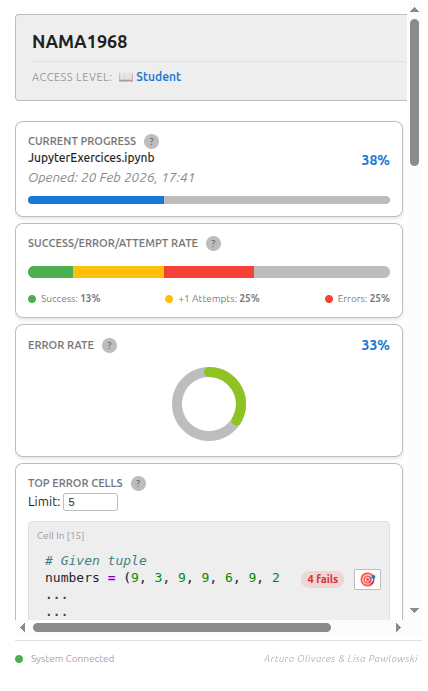
\includegraphics[scale=0.5]{img/Dashboard/general.png}
    \caption{General overview of the dashboard design.}
    \label{fig:dash:general}
    \Description{General overview of the dashboard design. The different panels of the dashboard are shown, including the user information panel, the current progress panel, the success/error/attempt rate panel, the error rate panel and the top error cells panel.}
\end{figure}
The dashboard is organized into different panels, each of which providing the students with relevant information. In addition to the visualizations, each panel includes a help button that provides a brief explanation of the information being presented and how it can be interpreted. The panels available in the dashboard are:
\begin{description}
    \item[User Information] (Figure~\ref{fig:dash:user_info}) This panel displays the user's personal code and their role.
    \begin{figure}
        \centering
        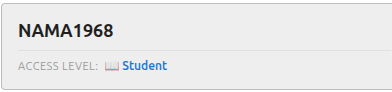
\includegraphics[scale=0.5]{img/Dashboard/user_info.png}
        \caption{User information panel.}
        \label{fig:dash:user_info}
        \Description{User information panel. The user's personal code and role are displayed.}
    \end{figure}

    \item[Current Progress] (Figure~\ref{fig:dash:current_progress}) This panel provides, apart from the title of the notebook and the opening time of the current notebook session, a visualization of the student's progress in the current notebook session. The progress is calculated as described in Equation~\eqref{eq:progress}.
    \begin{equation}\label{eq:progress}
        \text{Progress} = \frac{\text{Number of code cells with an execution without errors}}{\text{Total number of code cells}}
        \times 100\%
    \end{equation}
    \begin{figure}
        \centering
        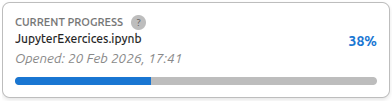
\includegraphics[scale=0.5]{img/Dashboard/current_progress.png}
        \caption{Current progress panel.}
        \label{fig:dash:current_progress}
        \Description{Current progress panel. The title of the notebook, the opening time of the current notebook session and a visualization of the student's progress in the current notebook session are displayed.}
    \end{figure}

    \item[Success/Error/Attempt Rate] (Figure~\ref{fig:dash:success_error_attempt_rate}) This panel provides a more detailed view of the student's progress. It classifies the code cells into three categories:
    \begin{itemize}
        \item Successful cells: code cells with only one execution, and that execution did not produce any errors.
        \item Attempted cells: code cells with more than one execution, having the last execution without errors.
        \item Error cells: code cells where the last execution produced an error.
    \end{itemize}
    The panel shows the rate of successful, attempted and error cells in the current notebook session, calculated as described in the Equation~\eqref{eq:rates}.
    \begin{equation}\label{eq:rates}
        \text{Rate} = \frac{\text{Number of cells in the category}}{\text{Total number of code cells}}
        \times 100\%
    \end{equation}
    \begin{figure}
        \centering
        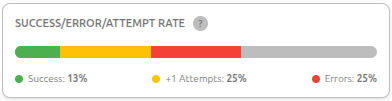
\includegraphics[scale=0.5]{img/Dashboard/success_error_attempt_rate.png}
        \caption{Success/Error/Attempt rate panel.}
        \label{fig:dash:success_error_attempt_rate}
        \Description{Success/Error/Attempt rate panel. The rate of successful, attempted and error cells in the current notebook session is displayed.}
    \end{figure}

    \item[Error Rate] (Figure~\ref{fig:dash:error_rate}) This panel focuses on the error rate in the current notebook session, calculated as described in Equation~\eqref{eq:error_rate}. It should be noted that the color used in the visualization changes according to the error rate, being green for $0\%$, red for $100\%$, and a gradient of colors in between for the values in between.
    \begin{equation}\label{eq:error_rate}
        \text{Error Rate} = \frac{\text{Number of executions with errors}}{\text{Total number of executions}}
        \times 100\%
    \end{equation}
    \begin{figure}
        \centering
        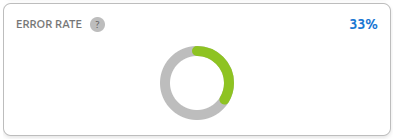
\includegraphics[scale=0.5]{img/Dashboard/error_rate.png}
        \caption{Error rate panel.}
        \label{fig:dash:error_rate}
        \Description{Error rate panel. The error rate in the current notebook session is displayed.}
    \end{figure}

    \item[Top Error Cells] (Figure~\ref{fig:dash:top_error_cells}) This panel shows the top $n$ code cells with the highest number of executions with errors in the current notebook session. The parameter $n$ can be configured by the user, allowing them to choose how many cells they want to see in this panel. The cells are ordered from the one with the highest number of executions with errors to the one with the lowest. For each cell, the panel displays the cell content of the last execution, the number of executions with errors, and a button that allows the user to jump to the cell in the notebook.
    \begin{figure}
        \centering
        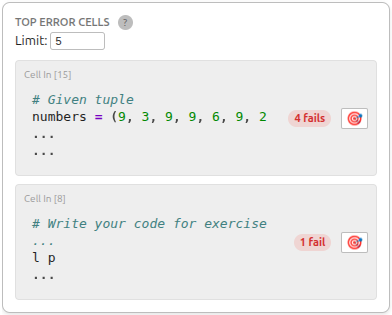
\includegraphics[scale=0.5]{img/Dashboard/top_error_cells.png}
        \caption{Top error cells panel.}
        \label{fig:dash:top_error_cells}
        \Description{Top error cells panel. The top error cells in the current notebook session are displayed.}
    \end{figure}

    \item[Top Attempt Cells] (Figure~\ref{fig:dash:top_attempt_cells}) This panel shows the top $n$ code cells with the highest number of executions in the current notebook session. For each cell, the panel displays the total number of executions.
    \begin{figure}
        \centering
        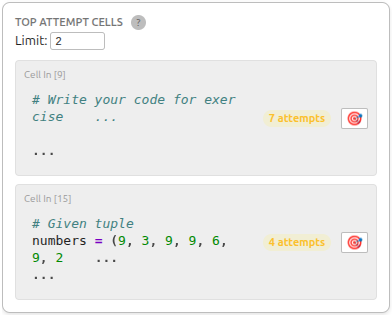
\includegraphics[scale=0.5]{img/Dashboard/top_attempt_cells.png}
        \caption{Top attempt cells panel.}
        \label{fig:dash:top_attempt_cells}
        \Description{Top attempt cells panel. The top attempt cells in the current notebook session are displayed.}
    \end{figure}

    \item[Top Time-Consuming Cells] (Figure~\ref{fig:dash:top_time_consuming_cells}) This panel shows the top $n$ code cells with the highest total execution time in the current notebook session. For each cell, the panel displays the total time that the cell has been active during the notebook session.
    \begin{figure}
        \centering
        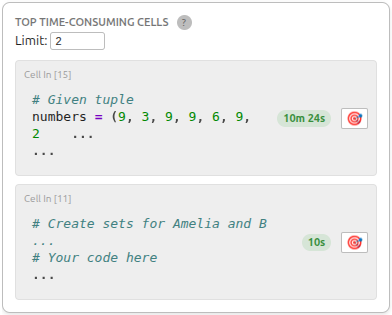
\includegraphics[scale=0.5]{img/Dashboard/top_time_consuming_cells.png}
        \caption{Top time-consuming cells panel.}
        \label{fig:dash:top_time_consuming_cells}
        \Description{Top time-consuming cells panel. The top time-consuming cells in the current notebook session are displayed.}
    \end{figure}

    \item[Top Common Error Types] (Figure~\ref{fig:dash:top_common_error_types}) This panel shows the top $n$ most common Python error types in the current notebook session, such as \texttt{IndexError}, \texttt{SyntaxError} or \texttt{NameError}. For each error type, the panel displays the number of occurrences of that error type.
    \begin{figure}
        \centering
        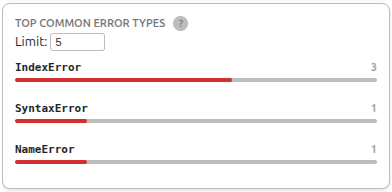
\includegraphics[scale=0.5]{img/Dashboard/top_common_error_types.png}
        \caption{Top common error types panel.}
        \label{fig:dash:top_common_error_types}
        \Description{Top common error types panel. The top common error types in the current notebook session are displayed.}
    \end{figure}

    \item[Execution Timeline] (Figure~\ref{fig:dash:execution_timeline}) This panel provides a timeline visualization of the code cell executions in the current notebook session. Each execution is represented as a point on the timeline, being the color of the point green if the execution was successful, and red if it produced an error. This visualization allows students to see the distribution of their successful and unsuccessful executions over time.
    \begin{figure}
        \centering
        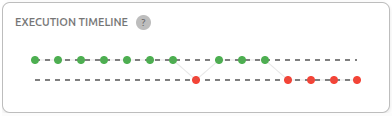
\includegraphics[scale=0.5]{img/Dashboard/execution_timeline.png}
        \caption{Execution timeline panel.}
        \label{fig:dash:execution_timeline}
        \Description{Execution timeline panel. The execution timeline in the current notebook session is displayed.}
    \end{figure}
\end{description}

\subsection{Survey Design}

The survey is designed to collect data on students' perceptions of the learner-facing dashboard in a Jupyter-based programming environment.

\subsubsection{Data Collection}

Before the data collection could start, the study was reviewed and approved by the Ethics Committee of the University of Duisburg-Essen. The ethics approval ID is 2601CMPL2910.
The data were collected via an online survey using LimeSurvey, in which participants could take part only once (see Appendix~\ref{sec:appendix_questionnaires}).
This standardized survey design ensured that all participants answered the questions in the same order in order to reduce potential confounding variables that might arise from differing procedures. In this way, a high level of replicability of the study could be ensured.

At the beginning of the study, participants were informed about the purpose of the study and the associated ethical aspects. It was made clear that participation was voluntary and that participants could withdraw from the study at any time without providing reasons or facing any consequences. Prior to starting the survey, participants were therefore required to give their informed consent. The questionnaire then began with initial questions regarding their previous experience with Jupyter Notebook and Python for comparison purposes. After that, the students began testing the Jupyter Dashboard while solving Python exercises.
Subsequently, questionnaires measuring usability and usefulness of the Jupyter Dashboard and a person's subjective mental workload by assessing six key dimensions such as mental demand, physical demand, temporal demand, performance, effort, and frustration level were administered.
This was followed by the collection of sociodemographic information, including age, gender, course of study and what semester the participants are in, in order to better describe and analyze the sample. A control question was added at the end to check whether the subjects had completed the questionnaire honestly and carefully. Finally, participants were informed about the further course of the study and thanked for their participation.

\subsubsection{Measurements}

The usability of the dashboard was assessed using the System Usability Scale (SUS)~\cite{germanupa_sus}. The SUS is a standardized and widely used instrument for evaluating the perceived usability of interactive systems. It consists of 10 items that capture users' subjective assessment of system usability, including aspects such as complexity, ease of use, and confidence in using the system. The items are rated on a 5-point Likert scale ranging from 1 (``strongly disagree'') to 5 (``strongly agree''). The scale includes five positively worded and five negatively worded items, requiring reverse coding of the negatively formulated statements prior to analysis. A sample item is: ``I thought the system was easy to use.'' The SUS score is calculated by converting item responses according to the standard scoring procedure and multiplying the sum by 2.5, resulting in a total score ranging from 0 to 100, with higher values indicating higher perceived usability. A score above 68 is commonly interpreted as indicating above-average usability. The SUS was chosen because it has demonstrated good reliability and validity across a wide range of domains and technologies with a Cronbach's Alpha $=.95$~\cite{chu2019usability}.

Perceived usefulness and acceptance of the dashboard were measured using constructs derived from the Technology Acceptance Model (TAM)~\cite{davis1989technology}. According to the model, individuals' intention to use a system is primarily determined by their perceived usefulness and perceived ease of use. Perceived usefulness refers to the extent to which a person believes that using a particular system enhances their performance, whereas perceived ease of use reflects the degree to which a person believes that using the system is free of effort. All items were rated on a 7-point Likert scale ranging from 1 (``extremely unlikely'') to 7 (``extremely likely''). Example items include statements such as ``Using the dashboard improves my learning performance'' and ``I find the dashboard easy to use.'' For each construct, mean scores were calculated by averaging the corresponding items, with higher values indicating stronger agreement. The TAM has been widely validated across technological and educational contexts and typically demonstrates good internal consistency for both dimensions with a Cronbach's Alpha $=.89$~\cite{masrom2007technology}.

Perceived workload associated with using the dashboard was assessed using the NASA Task Load Index~\cite{hart1988development}.
The NASA-TLX is a widely used multidimensional instrument for measuring subjective workload in human-computer interaction and learning environments. It captures the overall perceived task load across six dimensions: mental demand, physical demand, temporal demand, performance, effort, and frustration~\cite{hart1988development}.


\section{Results}
\subsection{Sample Characteristics}

Sample characteristics are available in Table~\ref{tab:sample_characteristics}. The final sample consisted of 22 students, including 9 female and 11 male participants, while 2 participants did not specify their gender. Participants' ages ranged from 21 to 28 years ($M = 25$, $SD = 2.145$). Thirteen participants reported prior experience with Jupyter Notebook. Self-reported Python proficiency was measured on a scale from 1 to 10 and showed a relatively even distribution across different levels of expertise, allowing the dashboard to be evaluated by students with varying programming backgrounds. The participants spent an average of $17.289$ minutes testing the dashboard.
\begin{table}
  \centering
  \caption{Sample Characteristics ($N=22$)}
  \label{tab:sample_characteristics}
  \small
  \begin{tabular}{@{} l l r @{}} 
    \toprule
    \textbf{Characteristic} & \textbf{Category / Metric} & {\textbf{Value}} \\
    \midrule
    \textbf{Gender}         & Female                & 9 ($40.9\%$) \\
                            & Male                  & 11 ($50.0\%$) \\
                            & Unspecified           & 2 ($9.1\%$) \\
    \addlinespace
    \textbf{Age (Years)}    & Mean (SD)             & $25.00$ ($2.15$) \\
                            & Range                 & {21--28} \\
    \addlinespace
    \textbf{Coding Knowledge} & Mean (SD)          & $4.82$ ($2.70$) \\
                            & Range                 & {0--9} \\
    \addlinespace
    \textbf{Testing Duration (min)} & Mean (SD)   & $17.29$ ($7.68$) \\
                            & Range                 & {3--34} \\
    \bottomrule
  \end{tabular}
\end{table}

\subsection{Reliability of Scales}
The internal consistency of the multi-item scales was assessed using Cronbach's alpha~\cite{cronbach1951coefficient}. The System Usability Scale demonstrated acceptable to good reliability ($\alpha = .794$). For the Technology Acceptance Model subscales, Perceived Usefulness achieved good reliability ($\alpha = .852$), and Perceived Ease of Use showed excellent reliability ($\alpha = .941$). These reliability estimates confirm that the scales are sufficiently consistent for the purposes of this study, despite the relatively small sample size ($N = 22$). No items were removed to improve alpha, as all contributed positively to their respective scales.

\subsection{Descriptive Statistics}
Descriptive statistics for all main study variables are presented in Table~\ref{tab:descriptive_stats}.
Participants ($N = 22$) rated the perceived usability of the dashboard with a mean SUS score of $M = 65.57$ ($SD = 17.89$, range $40-90$). This value falls slightly below the widely reported average SUS benchmark of 68, indicating usability in the lower-to-average range. The Technology Acceptance Model (TAM) overall score averaged $M = 5.36$ ($SD = 0.88$, range $3.25-6.75$) on a 7-point Likert scale. The subscale Perceived Usefulness (PU) had a mean of $M = 4.93$ ($SD = 1.18$), while Perceived Ease of Use (PEOU) was higher at $M = 5.78$ ($SD = 1.06$). These values suggest moderate-to-positive perceptions of usefulness and particularly ease of use.
The subjective mental workload (NASA-TLX) yielded a mean overall score of $M = 8.15$ ($SD = 2.92$, range $1.67-12.67$) on a scale of 0 to 20. This indicates a relatively low-to-moderate perceived workload~\cite{hertzum2021reference}. 
\begin{table}
  \centering
  \caption{Descriptive Statistics of Main Study Variables ($N=22$)}
  \label{tab:descriptive_stats}
  \small
  \begin{tabular}{l r r r r}
    \toprule
    \textbf{Construct} & \textbf{M} & \textbf{SD} & \textbf{Min} & \textbf{Max} \\
    \midrule
    System Usability Scale (SUS)   & 65.57 & 17.89 & 40.00 & 90.00 \\
    TAM Overall                    &  5.36 &  0.88 &  3.25 &  6.75 \\
    \quad Perceived Usefulness (PU)  &  4.93 &  1.18 &  3.33 &  7.00 \\
    \quad Perceived Ease of Use (PEOU) &  5.78 &  1.06 &  3.17 &  7.00 \\
    NASA-TLX (Mental Workload)     &  8.15 &  2.92 &  1.67 & 12.67 \\
    \bottomrule
  \end{tabular}
\end{table}

Distributions were largely symmetric with a skewness near 0 for SUS and overall TAM, with some negative skewness in PEOU and NASA-TLX, suggesting a slight tendency toward higher ratings in those scales. Kurtosis values were acceptable overall, with no extreme deviations from normality.
To explore the relationships between usability, technology acceptance, and cognitive workload, Spearman rank-order correlations were computed (see Table~\ref{tab:correlations}). Given the small sample size ($N = 22$) and the use of Likert-scale data, non-parametric correlations were deemed appropriate. As expected, the TAM subscales Perceived Usefulness ($\rho = .816$, $p < .001$) and Perceived Ease of Use ($\rho = .706$, $p < .001$) exhibited strong, positive, and statistically significant correlations with the overall TAM score. Beyond these internal TAM associations, the analyses did not reveal any statistically significant relationships between the main constructs ($p > .05$). Specifically, perceived cognitive workload (NASA-TLX) did not significantly correlate with overall technology acceptance ($\rho = .024$, $p = .914$) or system usability ($\rho = -.099$, $p = .661$). While there was a moderate positive trend between the System Usability Scale (SUS) and Perceived Ease of Use ($\rho = .406$), this association did not reach statistical significance ($p = .061$).


\begin{table}
  \centering
  \begin{threeparttable}
    \caption{Spearman Rank Correlations ($\rho$) Between Main Study Variables ($N=22$)}
    \label{tab:correlations}
    \small
    \begin{tabular}{l r r r r r}
      \toprule
      \textbf{Variable} & \textbf{1} & \textbf{2} & \textbf{3} & \textbf{4} & \textbf{5} \\
      \midrule
      1. SUS               & ---   &       &       &       &       \\
      2. PU (TAM)          & .091  & ---   &       &       &       \\
      3. PEOU (TAM)        & .406  & .222  & ---   &       &       \\
      4. TAM Overall       & .323  & .816\tnote{*} & .706\tnote{*} & ---   &       \\
      5. NASA-TLX          & -.099 & .239  & -.255 & .024  & ---   \\
      \bottomrule
    \end{tabular}
    \begin{tablenotes}
      \footnotesize
      \item[*] $p < .001$, so these correlations are statistically significant.
    \end{tablenotes}
  \end{threeparttable}
\end{table}

\section{Discussion}
\subsection{Interpretation of Results}
The primary objective of this study was to evaluate the usability, perceived usefulness, and cognitive workload of a student-facing JupyterLab dashboard designed to visualize fine-grained notebook interactions. The results provide a differentiated perspective on how students perceive learner-facing analytics tools in programming contexts and allow the findings to be situated within the broader literature on notebook analytics and learning dashboards.
\subsubsection{RQ 1: Usability}
The mean SUS score of $M=65.57$ indicates that the system is marginally acceptable according to established benchmarks. While this score falls just short of the above average threshold of 68, it is important to contextualize this within the internal consistency of the scale $\alpha=.794$. The gap between the observed score and the benchmark suggests that while the core functionality is present, the integration of complex interaction data, such as cell execution histories and error patterns, into a single dashboard may require further UI refinement to reduce perceived complexity. Qualitative feedback from participants explicitly illustrated these interface constraints. For instance, one student suggested that ``in top error cells it might be better if it could show error lines in the code and in the dashboard.'' This highlights a clear user desire for tighter visual integration between the analytics and the active coding area. Furthermore, one potential factor contributing to the SUS score falling slightly below the average threshold relates to the dashboard's layout and information density. Due to limited screen real estate, participants were required to scroll vertically to access all visualizations. This necessity for scrolling and searching for information can increase the cognitive burden on users, a challenge that learning analytics tools must actively avoid to be effective~\cite{corrin2014exploring}. Transitioning to a single-page layout that presents all summary statistics and timelines simultaneously would align better with the established design principle of perceiving learning at a glance~\cite{schwendimann2016perceiving}. Such a redesign could enhance clarity, reduce navigational effort, and potentially lead to higher technology acceptance and usability ratings.

\subsubsection{RQ 2: Usefulness and Ease of Use}
A compelling contrast emerged between the TAM subscales. Participants rated the Perceived Ease of Use (PEOU) significantly higher $M = 5.78$ than the Perceived Usefulness (PU) $M = 4.93$. The excellent reliability of the PEOU scale $\alpha = .941$ underscores that the dashboard itself is perceived as intuitive and easy to navigate. These findings strongly align with existing literature on learning analytics. The high PEOU score demonstrates that the dashboard successfully meets the requirement outlined by Corrin and De Barba~\cite{corrin2014exploring}, who emphasize that reflection tools must be seamlessly integrated without increasing cognitive burden. However, the more moderate PU score reflects a well-documented challenge in the field as Corrin and De Barba~\cite{corrin2014exploring} also note, students often require time and guidance to effectively interpret analytics feedback. While the dashboard visualizes the fragmented workflows and trial-and-error strategies described by Robinson et al.~\cite{robinson2022error}, recognizing the metacognitive value of these visualizations as advocated by Schwendimann et al.~\cite{schwendimann2016perceiving} likely requires longitudinal engagement beyond a 17-minute testing session. Qualitative feedback strongly supported this discrepancy between ease of use and perceived usefulness. Multiple participants expressed that the tool currently feels more aligned with an instructor's perspective, with one student noting, ``I feel like the dashboard is more of data analysis rather than for the student itself.'' Another participant explicitly requested actionable guidance, stating: ``I think it would be more useful for a teacher. I think it would be more useful for students to see how to solve a specific error, instead of just getting the feedback which errors you made.'' This directly echoes existing research on notebook-based analytics tools, which suggests that while fine-grained interaction data can reveal important workflow insights, learners may initially perceive such transparency as descriptive rather than transformative~\cite{cai2025jupyter,JELAI}. In other words, students may recognize that the dashboard shows them what they did, but may not yet connect this information to improved future performance without explicit instructional tips. Interestingly, despite these reservations about general usefulness, students did identify specific situational benefits. As one learner pointed out, ``I think this dashboard is useful when the learner wants to do a coding exam, so they know how much time they spent on one task,'' indicating that the perceived value of the tool may depend on the specific educational context.

\subsubsection{Overall User Experience and Workload}
Although not explicitly bound to a singular research question, assessing the subjective mental workload was a fundamental component in evaluating the dashboard's overall viability. A central and highly positive finding of this study is the low subjective mental workload measured via the NASA Task Load Index (NASA-TLX), which yielded a mean overall score of $M = 8.15$ ($SD = 2.92$) on a 20-point scale. When linearly transformed to a 100-point scale (approx. $40.75$), this value sits comfortably below the global median of $43.8$ reported in comprehensive user-experience meta-analyses~\cite{hertzum2021reference}.
This result directly addresses a critical concern in the design of educational tools. Computational notebooks already present a dense interactive structure by mixing narrative text, code, and visual output. Introducing an additional layer of fine-grained analytics inherently risks overwhelming the user. However, the low NASA-TLX score strongly suggests that the dashboard fulfills the critical requirement of being a low-workload addition to the programming environment. As emphasized by Corrin and De Barba~\cite{corrin2014exploring}, for learning analytics tools to be genuinely effective, they must be seamlessly integrated into the student's workflow without increasing cognitive burden.
The workload findings confirm that the dashboard successfully avoids this ``cognitive burden'' trap. It provides students with transparent, cell-level execution histories and visual timelines without distracting them from their primary goal of solving Python exercises. In combination with the high Perceived Ease of Use (PEOU) reported in RQ2, these results indicate that while students may still need pedagogical guidance to translate the dashboard's descriptive data into actionable steps, the system itself does not impose a significant cognitive hurdle. This lays a robust foundation for future iterations to focus on enhancing the instructional value of usefulness without needing to overhaul the underlying interaction paradigm.

\subsection{Limitations}
While this study provides valuable initial insights into the usability and acceptance of a learner-facing Jupyter dashboard, several limitations must be acknowledged. First, the sample size of 22 students restricts the generalizability of the findings and the statistical power necessary to detect significant correlations between perceived workload, usability, and technology acceptance. Although the sample size was sufficient for an exploratory evaluation and the scales demonstrated acceptable to excellent internal consistency, a larger and more diverse sample size would be required to draw robust, population-level conclusions. In addition to that, the short duration of the testing phase represents a significant constraint. Participants interacted with the dashboard while solving Python exercises for an average of approximately 17 minutes. As discussed regarding the moderate Perceived Usefulness scores, developing metacognitive skills and recognizing the instructional value of workflow reflection often requires long-term engagement and explicit pedagogical assistance~\cite{corrin2014exploring}. The brief exposure in this study captures initial impressions but may not accurately reflect how students would perceive, integrate, and benefit from the dashboard over the course of an entire academic semester.

\subsection{Future Work}
Building upon the foundational usability and technology acceptance findings of this exploratory study, future research should transition from subjective user evaluations to measuring objective pedagogical outcomes. A promising direction for subsequent research would be to conduct controlled experimental studies comparing learners with and without access to the dashboard over multiple learning units. Such studies could investigate whether providing visual feedback on cell execution histories, error rates, and time spent on tasks directly translates into improved programming performance. Researchers could focus on quantifying performance improvements through metrics such as the reduction in error rates between coding sessions, increased execution efficiency e.g., fewer retries per cell, and overall task correctness. To further refine the assessment of execution efficiency, future iterations of the system could utilize specific cell execution durations to evaluate whose code is more computationally optimized. Additionally, to accurately measure overall task correctness, the dashboard should integrate a database of verified solutions. Currently, code that executes without triggering an exception may be interpreted as successful, cross-referencing outputs with a validated database would allow the system to distinguish between code that merely executes without errors and code that is functionally correct.
Furthermore, to better understand the mechanisms of self-regulated learning, future iterations could integrate explicit reflection prompts directly into the dashboard interface. By combining system logs with pre- and post-surveys measuring variables like programming self-efficacy and motivation, researchers could determine whether increased metacognitive awareness actively mediates problem-solving success. 
Finally, while the current project focused exclusively on a student-facing dashboard, future work should expand this concept by developing and evaluating an instructor-facing counterpart. Gathering qualitative and quantitative feedback from educators will be essential to understand how aggregating this fine-grained student interaction data could facilitate targeted pedagogical interventions and reveal common coding difficulties across an entire cohort. Expanding these analytics to include direct comparisons between different students could provide both instructors and learners with valuable benchmarking insights, highlighting diverse problem-solving approaches and helping educators identify outliers who may need additional support or advanced challenges.

\section{Conclusion}
As programming becomes increasingly integrated into scientific and educational workflows, understanding how students interact with computational notebooks is of crucial importance. This study evaluated a JupyterLab dashboard extension designed to monitor notebook activity and make the iterative, trial-and-error nature of programming transparent to learners. The evaluation demonstrated that while translating complex, cell-level interaction data into an intuitive user interface presents certain layout and usability challenges, the underlying concept is highly viable. Students perceived the dashboard as very easy to use and reported a low subjective mental workload. This is a key success, as it indicates that the system effectively avoids creating additional cognitive hurdles during programming. Although recognizing the immediate instructional usefulness of these visualizations likely requires more longitudinal engagement, targeted pedagogical guidance, and the integration of concrete problem-solving hints, the dashboard lays an important foundation. By shifting away from purely outcome-based evaluations toward process-oriented analytics, tools like this have the potential to sustainably bridge the gap between the correctness of the final code and the students' individual learning paths.

%%
%% The next two lines define the bibliography style to be used, and
%% the bibliography file.
\newpage
\nocite{*}
\bibliographystyle{ACM-Reference-Format}
\bibliography{sample-base}

\newpage
\appendix
\counterwithin{table}{section}
\counterwithin{figure}{section}

\section{Learning Analytics Model}

\begin{figure}[H]
  \centering
  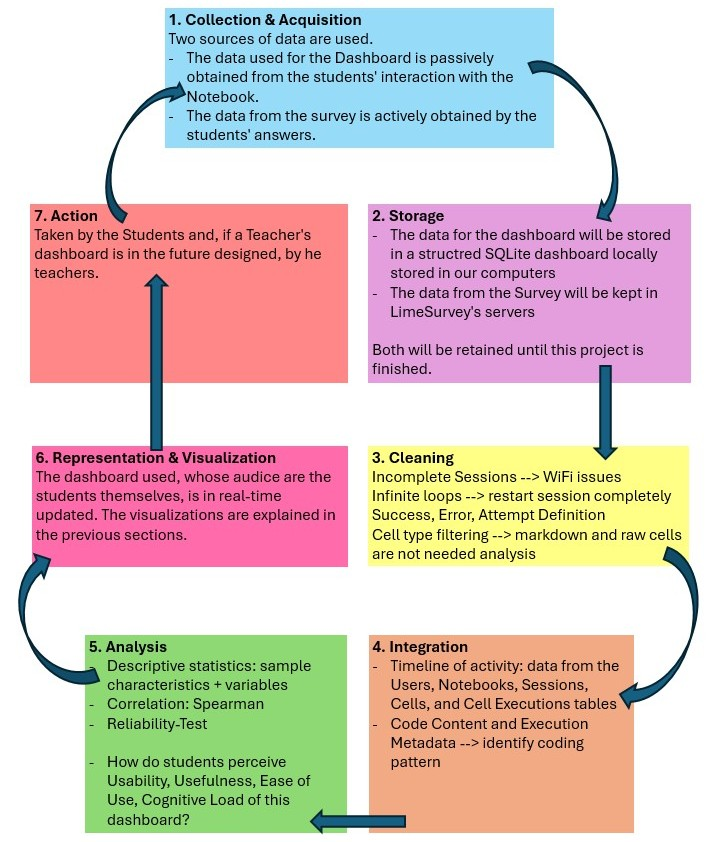
\includegraphics[width=\textwidth]{./img/LAM.jpg}
  \caption{Learning Analytics Model for this project.}
  \Description{A diagram illustrating the Learning Analytics Model (LAM) used in this project, showing the flow from data collection to analysis and feedback.}
  \label{fig:learning_analytics_model}
\end{figure}

\section{Questionnaire Items}
\label{sec:appendix_questionnaires}
This appendix provides the exact wording of the items used in the evaluation survey to measure system usability, technology acceptance, and perceived cognitive workload.

\subsection{System Usability Scale (SUS)}
Participants rated the following 10 items on a 5-point Likert scale (1 = Strongly Disagree to 5 = Strongly Agree). 

\begin{table}[htpb]
  \centering
  \caption{Items of the System Usability Scale (SUS)}
  \label{tab:app_sus}
  \begin{tabular}{lp{0.85\linewidth}}
    \toprule
    \textbf{Item} & \textbf{Statement} \\
    \midrule
    SUS01 & I think I would like to use this Dashboard frequently. \\
    SUS02 & I found this Jupyter Dashboard unnecessarily complex. \\
    SUS03 & I thought the Jupyter Dashboard was easy to use. \\
    SUS04 & I think that I would need the support of a technical person to use the Jupyter Dashboard. \\
    SUS05 & I found the various functions in this dashboard were well integrated. \\
    SUS06 & I thought there was too much inconsistency in this dashboard. \\
    SUS07 & I would imagine that most people would learn to use this dashboard very quickly. \\
    SUS08 & I found this dashboard very awkward to use. \\
    SUS09 & I felt very confident using this Jupyter Dashboard. \\
    SUS10 & I needed to learn a lot of things before I could get going with this dashboard. \\
    \bottomrule
  \end{tabular}
\end{table}

\subsection{Technology Acceptance Model (TAM)}
Participants rated the TAM items on a 7-point Likert scale (Extremely Unlikely to Extremely Likely). The construct was divided into Perceived Usefulness (PU) and Perceived Ease of Use (PEOU).

\begin{table}[htpb]
  \centering
  \caption{Items of the Technology Acceptance Model (TAM)}
  \label{tab:app_tam}
  \begin{tabular}{lp{0.85\linewidth}}
    \toprule
    \textbf{Construct} & \textbf{Statement} \\
    \midrule
    \textbf{PU} & \textit{Using the Jupyter Dashboard to assist my learning progress would...} \\
    PU01 & ...enable me to accomplish tasks more frequently. \\
    PU02 & ...improve my learning performance. \\
    PU03 & ...increase my productivity. \\
    PU04 & ...enhance my effectiveness during the task. \\
    PU05 & ...make it easier to do my tasks. \\
    PU06 & ...be useful. \\
    \midrule
    \textbf{PEOU} & \textit{How much do you agree with each statement?} \\
    PEOU01 & Learning to operate this Dashboard would be easy for me. \\
    PEOU02 & I would find it easy to get this Dashboard to do what I want it to do. \\
    PEOU03 & My interaction with the Dashboard would be clear and understandable. \\
    PEOU04 & I would find this Dashboard would be clear and understandable. \\
    PEOU05 & It would be easy for me to become skillful at using this Dashboard. \\
    PEOU06 & I would find this Dashboard easy to use. \\
    \bottomrule
  \end{tabular}
\end{table}

\subsection{NASA Task Load Index (NASA-TLX)}
Participants rated the following items on a continuous scale from 0 to 20 to measure their perceived workload during the task.

\begin{table}[htpb]
  \centering
  \caption{Items of the NASA-TLX}
  \label{tab:app_nasatlx}
  \begin{tabular}{lp{0.85\linewidth}}
    \toprule
    \textbf{Dimension} & \textbf{Question} \\
    \midrule
    Mental Demand & How mentally demanding was the task? \\
    Physical Demand & How physically demanding was the task? \\
    Temporal Demand & How hurried or rushed was the pace of the task? \\
    Performance & How successful were you in accomplishing what you were asked to do? \\
    Effort & How hard did you have to work to accomplish your level of performance? \\
    Frustration & How insecure, discouraged, irritated, stressed, and annoyed were you? \\
    \bottomrule
  \end{tabular}
\end{table}






\end{document}
\endinput
%%
%% End of file `sample-manuscript.tex'.